\documentclass[12pt]{beamer}
\usetheme{Warsaw}
\usepackage[utf8]{inputenc}
\usepackage[english]{babel}
\usepackage{amsmath}
\usepackage{stmaryrd}
\usepackage{amsfonts}
\usepackage{amssymb}
\usepackage{graphicx}
\usepackage{xcolor}
\usepackage[backend=bibtex, style=authoryear, maxcitenames=2]{biblatex}
\addbibresource{../../Thesis/references.bib} 
\renewcommand*{\bibfont}{\footnotesize}
\usepackage{url}
\definecolor{lila}{RGB}{128,0,128}

\newcommand{\myCite}[1]{{\scriptsize\parencite{#1}}}

\setbeamertemplate{navigation symbols}{}
\setbeamertemplate{footline}{%
	\raisebox{5pt}{%
		\makebox[\paperwidth]{%
			\hfill\makebox[10pt]{%
				\textcolor{gray}{\footnotesize\insertframenumber}
			}
		}
	}
}

\definecolor{regal}{RGB}{81,0,0}
\usepackage{array}
\usepackage{colortbl}
\makeatletter
\newcommand{\thickhline}{%
    \noalign {\ifnum 0=`}\fi \color{regal}\hrule height 4pt
    \futurelet \reserved@a \@xhline
}
\newcolumntype{"}{@{\color{regal}\hskip\tabcolsep\vrule width 8pt\hskip\tabcolsep}}
\makeatother

% listings
\usepackage[TS1,T1]{fontenc}
\usepackage{newunicodechar}
\newcommand*\longs{{\fontencoding{TS1}\selectfont s}}
\newunicodechar{ſ}{\longs}
\usepackage{listings}
\definecolor{mygreen}{rgb}{0,0.6,0}
\definecolor{mygray}{rgb}{0.5,0.5,0.5}
\definecolor{mymauve}{rgb}{0.58,0,0.82}
\lstset{
	captionpos=b,
	frame=single,
	breaklines=true,
	breakatwhitespace=true,
	literate=%
		{Ö}{{\"O}}1
		{Ä}{{\"A}}1
		{Ü}{{\"U}}1
		{ß}{{\ss}}1
		{ü}{{\"u}}1
		{ä}{{\"a}}1
		{ö}{{\"o}}1
		{~}{{\textasciitilde}}1,
	tabsize=4,
	aboveskip=4pt,
	belowskip=6pt,
	backgroundcolor=\color{white},   % choose the background color
	basicstyle=\footnotesize,        % size of fonts used for the code
	breaklines=true,                 % automatic line breaking only at whitespace
	captionpos=b,                    % sets the caption-position to bottom
	commentstyle=\color{mygreen},    % comment style
	escapeinside={\%*}{*)},          % if you want to add LaTeX within your code
	keywordstyle=\color{blue},       % keyword style
	stringstyle=\color{mymauve},     % string literal style
}
\definecolor{maroon}{rgb}{0.5,0,0}
\definecolor{darkgreen}{rgb}{0,0.5,0}
\lstdefinelanguage{XML}
{
	basicstyle=\ttfamily\tiny,
	morestring=[s]{"}{"},
	morecomment=[s]{?}{?},
	morecomment=[s]{!--}{--},
	commentstyle=\color{darkgreen},
	moredelim=[s][\color{black}]{>}{<},
	moredelim=[s][\color{red}]{\ }{=},
	stringstyle=\color{blue},
	identifierstyle=\color{maroon}
}

%\setbeamercovered{transparent} 
%\logo{}  
%\subject{} 
\begin{document} 
		
\begin{frame}[plain,noframenumbering]
	\begin{minipage}{0.1\textwidth}
		\hspace{-0.5cm}
\includegraphics[scale=0.049]{Images/Buchruecken}
	\end{minipage}
	\begin{minipage}{0.6\textwidth}
		\begin{center}
			\vspace{-1.5cm}
			\Large{Extracting recipe ingredients \\ from cookbooks} \\
			\vspace{0.5cm}
			\large{Heraus aus dem Sumpf} \\
			\small{von \\ \vspace{-0.1cm} Torsten Knauf}
		\end{center}
	\end{minipage}
	\begin{minipage}{0.25\textwidth}
		\arrayrulecolor{red}
		\small
		\begin{tabular}{"l}
			Der Beginn einer \\ Master-Arbeit \\
			\thickhline
			\color{white} \\
			Irrlichter \\
			\thickhline 
			\color{white} - \\
			\color{white} - \\
			\thickhline 
			\color{white} - \\
			\color{white} - \\
			\thickhline 
			\color{white} - \\
			\color{white} - \\
			\thickhline 
			\color{white} - \\
			\color{white} - \\
			\thickhline 
			\color{white} - \\
			\color{white} - 
		\end{tabular}
	\end{minipage}
\end{frame}


\begin{frame}[fragile]{Beispiel cueML}
	\begin{lstlisting}[language=XML]
<cue:recipe type="Suppen." rcp-id="B-16">
	<head>Mock Turtle Suppe.</head>
	
	<p>Es wird hierzu für <cue:yield atLeast="24" atMost="30">24-30 Personen</cue:yield> eine kräftige <ref target="#Bouillon">Bouillon</ref> von 8-10 Pfund <cue:recipeIngredient ref="#Rindkochfleisch" atLeast="8" atMost="10" unit="Pfund">Rindfleisch</cue:recipeIngredient> mit <cue:recipeIngredient ref="#Wurzelwerk">Wurzelwerk </cue:recipeIngredient> gekocht. [...]</p>
	
	<note>Anmerk. Der <cue:recipeIngredient ref="#Englische_Soja" optional="True">Soja</cue:recipeIngredient> macht die Suppe gewürzreicher, kann jedoch gut wegbleiben, und statt <cue:recipeIngredient ref="#Madeira" altGrp="1">Madeira</cue:recipeIngredient> kann man <cue:recipeIngredient ref="weißen_Franzwein" altGrp="2">weißen Franzwein</cue:recipeIngredient> und etwas <cue:recipeIngredient ref="#Rum" altGrp="2" quantity="etwas">Rum</cue:recipeIngredient> nehmen<cue:alt target="1 2"/>. Sowohl die Bouillon als Kalbskopf können schon am vorhergehenden Tage, ohne Nachtheil der Suppe, gekocht werden.</note>
</cue:recipe>
	\end{lstlisting}
\end{frame}

\begin{frame}[fragile]{Wie man es hätte auch machen können I}
	\begin{lstlisting}[language=XML]
	<...>
	und statt <cue:recipeIngredient ref="#Madeira" altGrp="1">Madeira</cue:recipeIngredient> kann man <cue:recipeIngredient ref="weißen_Franzwein" altGrp="2">weißen Franzwein</cue:recipeIngredient> und etwas <cue:recipeIngredient ref="#Rum" altGrp="2" quantity="etwas">Rum</cue:recipeIngredient> nehmen <cue:alt target="1 2"/>.
	
		VS
	
	und statt <recipeIngredient ref="#Madeira" xml:id="B-16-Madeira">Madeira</recipeIngredient> kann man <recipeIngredient ref="weißen_Franzwein" xml:id="B-16-Franzwein">weißen Franzwein</recipeIngredient> und etwas <recipeIngredient ref="#Rum" xml:id="B-16-Rum">Rum</recipeIngredient> nehmen. Sowohl die Bouillon als Kalbskopf können schon am vorhergehenden Tage, ohne Nachtheil der Suppe, gekocht werden.
	
	<recipeIngredientGrp xml:id="B-16-alt1" target="#B-16-Madeira"/>
	<recipeIngredientGrp xml:id="B-16-alt2" target="#B-16-Franzwein #B-16-Rum"/>
	<alt target="#B-16-alt1 #B-16-alt2" mode="excl"/>
	\end{lstlisting}
\end{frame}

\begin{frame}[fragile]{Wie man es hätte auch machen können II}
	\begin{lstlisting}[language=XML]
	<...>
	8-10 Pfund <cue:recipeIngredient ref="#Rindkochfleisch" atLeast="8" atMost="10" unit="Pfund">Rindfleisch</cue:recipeIngredient>
	
	VS
	
	<atLeast target="#Suppenrindfleisch">8</atLeast>-<atMost target="#Suppenrindfleisch">10</atMost> <unit target="#Suppenrindfleisch">Pfund</unit> <recipeIngredient ref="#Suppenrindfleisch">Rindfleisch</recipeIngredient>
	\end{lstlisting}
	
	\begin{center}
		\textcolor{red}{\Large{$\lightning$}}
	\end{center}
	Für quantity-Attribut \textit{ref="\#EINS"} für \textit{eine} \\
	Für unit-Attribut \textit{ref="\#MaßDef"} für \textit{Maß}
\end{frame}


\begin{frame}[fragile]{1. CRF Prototyp :)}
	\vspace{-0.7em}\begin{lstlisting}
für			...	O
24			... B-Yield
-			... I-Yield
30			... I-Yield
Personen	...	I-Yield
kräftige	... O
Bouillon	... O
von			...	O
8			...	B-Quantity
-			...	I-Quantity
10			...	I-Quantity
Pfund		...	B-Unit
Rindfleisch	... B-Ingredient
mit			...	O
Wurzelwerk	...	B-Ingredient
gekocht		...	O
.			...	O
	\end{lstlisting}
\end{frame}	

\begin{frame}
	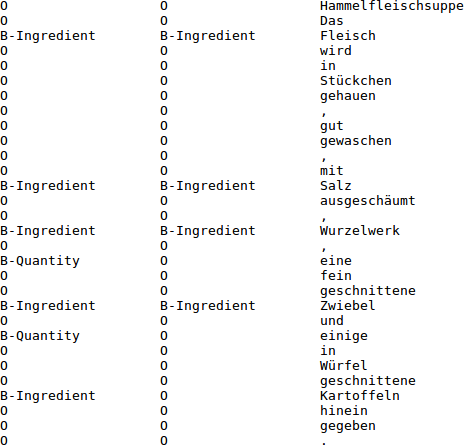
\includegraphics[scale=0.9]{Images/crfPrototypTagging}
\end{frame}

\begin{frame}
	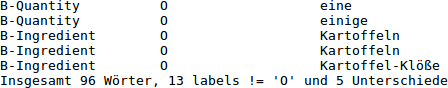
\includegraphics[scale=0.9]{Images/crfPrototypUnterschiede}
\end{frame}

\begin{frame}{Was noch fehlt}
	\begin{itemize}
		\item \textcolor{blue}{$\lightning$ \textit{optional="True"}}
		
		\item \textcolor{blue}{$\lightning$ \textit{altGrp="x"}}
		
		\item "Das Kalbfleisch wie in No. 1, nach der Personenzahl, doch etwas reichlicher genommen, da solches weniger Kraft gibt, als Rindfleisch." \textcolor{blue}{$\lightning$ \large\textit{dontUse="True"}}
		
		\item[\Large$\Rightarrow$] Label \& Feature Engineering
		\begin{itemize}
			\item Neue Labels: OptionalIngredient, AlternativeIngredient, DontUseIngredient
			\item Features: w[-1], w[-2], w[1], w[2], ...
			\item Noch mehr Labels und bigram-Features: "statt"/"oder" $\rightarrow$ IndicatorForAlternativeIngredient, "kann" $\rightarrow$ IndicatorForOptionalIngredient, ... 
		\end{itemize}
	\end{itemize}
\end{frame}

\begin{frame}{Was dann noch immer fehlt}
	\begin{itemize}
		\item ist altGrp \textcolor{blue}{$\lightning$ \textit{aber altGrp $\overset{!}{=}$ x}}
		
		\item "Rindfleischsuppe [...] das Fleisch" \textcolor{blue}{$\lightning$ \textit{implizite Informationen; ref $\overset{!}{=}$ x}}
		
		\item "8-10 Pfund Rindfleisch"\\
		$\rightarrow$ "B-Quantity O B-Quantity B-Unit B-Ingredient"\\
		\textcolor{blue}{$\lightning$ \textit{Zuordnung von Unit und Quantity}}
	\end{itemize}
\end{frame}

\begin{frame}{Ist CRF überhaupt der richtige Ansatz? :/}
	\begin{itemize}
		\item NYT betrachten nur Zeilen aus Zutatenliste \& hatten bereits über 130.000 gelabelte Trainingsdaten
		\item Labeln ist sehr aufwändig (10 Rezepte $\rightarrow$ 1514 Zeilen $\rightarrow$ 1514/60*3 $\rightarrow$ ca. 1.5h bis zu 3h)
		\item Wie gut wird das CRF sein?
	\end{itemize}
\end{frame}


\begin{frame}[fragile]{Alternativer Ansatz}
	\begin{enumerate}
		\item Lemmatisierung
		\item Dictionary-based Extraktion von Ingredients, Quantities, Units
		\item Rule-based Entity Processing
		\begin{lstlisting}[language=Python]
if "kann" in sentence:
	# add "optional='True'" to Ingredient

if "statt" in sentence:
	# add "altGrp='id1'" to first ingredient
	# add "altGrp='id2'" to following ingredients  
	
if ingredient == "Fleisch" and
		recipe.Name.find("Rind") != -1:
	# ingredient = Rindfleisch
if ingredient == "Rindfleisch" and
		recipe.rcpId == "Suppe":
	# ingredient = Suppenrindfleisch
		\end{lstlisting}
	\end{enumerate}
\end{frame}


\begin{frame}{Brainstorming CRF vs. Rule-based Entity Processing}
	\begin{itemize}
		\item 8-10
		\item optional Ingredient
		\vspace{0.5cm}
		\item Link target?
		\item Zuordnungen von altGrps, Quantity / Unit / Ingredients nicht via CRF
		\item Rule-based schneller zu entwickeln und gezielter testbar / steuerbar (Feature, Labels, Trainingsdaten -> ?, Rules ändern -> Unit tests :) )
	\end{itemize}
\end{frame}

	
\begin{frame}
	\begin{minipage}{0.2\textwidth}
		\begin{center} \Large
			Happy\\
			about\\
			ALL\\
			kind\\
			of\\
			feedback\\
			
		\end{center}			
	\end{minipage}
	\begin{minipage}{0.65\textwidth}
		\hspace{2cm}
\includegraphics[scale=0.7]{Images/Recipes-are-like-a-dating-service}
	\end{minipage}
\end{frame}

\end{document}